\documentclass{article}
\usepackage{amsmath, amssymb, graphicx}
\usepackage{tikz}
\usetikzlibrary{positioning}

\begin{document}

\begin{figure}[h]
    \centering
    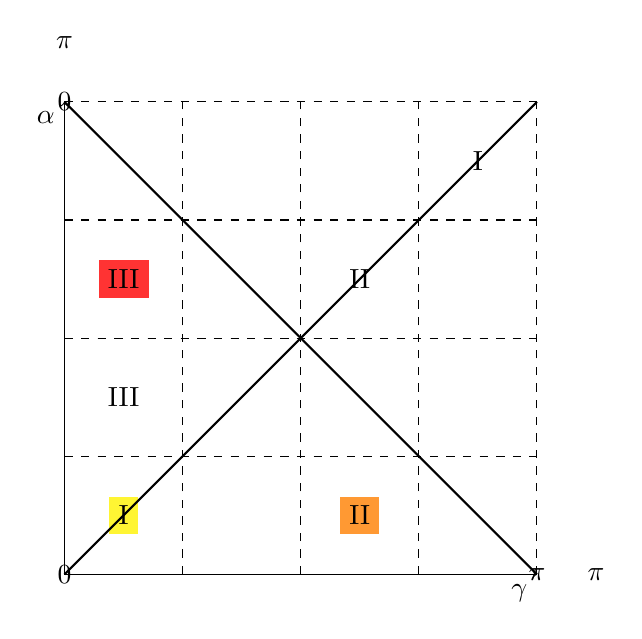
\begin{tikzpicture}[scale=1.5]
        % Axes
        \draw[->] (0,0) -- (4,0) node[below left] {$\gamma$};
        \draw[->] (0,0) -- (0,4) node[below left] {$\alpha$};
        
        % Grid lines
        \foreach \x in {0,...,4} \draw[dashed] (\x,0) -- (\x,4);
        \foreach \y in {0,...,4} \draw[dashed] (0,\y) -- (4,\y);
        
        % Labels
        \node at (0.5,0.5) [fill=yellow!80] {I};
        \node at (2.5,0.5) [fill=orange!80] {II};
        \node at (0.5,2.5) [fill=red!80] {III};
        
        % Phase boundaries
        \draw[thick] (0,0) -- (4,4);
        \draw[thick] (0,4) -- (4,0);
        
        % Dashed line
        \draw[dashed] (0,2) -- (4,2);
        
        % Annotations
        \node at (4.5,0) {$\pi$};
        \node at (0,4.5) {$\pi$};
        \node at (0,0) {$0$};
        \node at (4,0) {$\pi$};
        \node at (0,4) {$0$};
        \node at (3.5,3.5) {I};
        \node at (2.5,2.5) {II};
        \node at (0.5,1.5) {III};
    \end{tikzpicture}
    \caption{Phase diagram of the staggered six-vertex model with (quasi-)periodic boundary conditions in the critical regime with anisotropy $0 < \gamma \leq \pi$ \cite{FrMa12,KoLu23}. Lines with fixed staggering parameters $\alpha$ and $\pi - \alpha$ are identified by the duality transformation (\ref{ntjfn}). In phase I the scaling limit is described by a compact free boson -- as in the homogeneous limit $\alpha \to 0$. The critical degrees of freedom in phase II are one massless compact boson and two Majorana fermions. In phase III the low energy excitations of the model have been identified with those of the black hole coset model with a non-compact degree of freedom.}
    \label{fig:phase_diagram}
\end{figure}

\end{document}